\documentclass[10pt]{beamer}
\usetheme{Montpellier}

\usepackage{xspace, alltt}

\newcommand{\TODO}[2][]{[\textcolor{red}{TODO (#1):} \emph{#2}]}
\newcommand{\coq}{Coq\xspace}
\newcommand{\coqdoc}{Coqdoc\xspace}
\newcommand{\coqmakefile}{\texttt{coq\_makefile}\xspace}
\newcommand{\community}{Coq-community\xspace}
\newcommand{\gaia}{Gaia\xspace}
\newcommand{\alectr}{Alectryon\xspace}
\newcommand{\equations}{Equations\xspace}
\newcommand{\Hydras}{Hydras \& Co$\text.$\xspace}
\newcommand{\make}{\texttt{make}\xspace}


\definecolor{plugincolor}{rgb}{0.6,0.0,0.6}
\definecolor{mathcolor}{rgb}{0.0,0.0,0.6}
\definecolor{coqstylecolor}{rgb}{0.0,0.0,01.0}
\definecolor{lightblue}{rgb}{0.2,0.2,1.0}
\definecolor{metavarcolor}{rgb}{0.5,0.0,1.0}
\definecolor{darkgreen}{rgb}{0.1,0.7,0.1}
\definecolor{answercolor}{rgb}{.08,.15,.8}
\definecolor{normalcolor}{rgb}{0.0,0.0,0.0}
\definecolor{exbluecolor}{rgb}{0.1,0.1,0.9}
\definecolor{dontlookcolor}{rgb}{0.5,0.5,0.5}
\definecolor{termcolor}{rgb}{0.0,0.1,0.9}
\definecolor{lookcolor}{rgb}{0.9,0.1,0.0}
\definecolor{prooftermcolor}{rgb}{0.3,0.1,1.0}
\definecolor{typecolor}{rgb}{1.0,0.6,0.0}
\definecolor{taccolor}{rgb}{0.70,0.10,0.0}
\definecolor{pink}{rgb}{0.8,0.6,0.6}
\definecolor{darkmagenta}{rgb}{0.4,0.0,0.6}
\definecolor{darkblue}{rgb}{0.0,0.0,0.6}

\usepackage{tikz}
\usepackage{tikzsymbols}
\usepackage{pifont}
\usetikzlibrary{arrows}

\usepackage{ifpdf}
\ifpdf
\usepackage{graphicx}
%\usepackage{aeguill}
\else
\usepackage[dvips]{graphicx}
\fi


%%%%%%%%%%%%%%%%%%%%%%%%%%%%%%%%%%%%%%%%%%%%%%%%%%%%%%%%%%%%%%
%%%% For Alectryon

\usepackage{texments}
%%% for movies by alectryon
\usepackage{./alectryon}
\usepackage{../pygments}

% Prevent breaks in the middle of syntactic units
\let\OldPY\PY
\def\PY#1#2{\OldPY{#1}{\mbox{#2}}}


%%% One hypothesis per line 
\makeatletter
\renewcommand{\alectryon@hyps@sep}{\alectryon@nl}
\makeatother

%%% \snippets{A,B,C,…} inputs a series of snippets as one block (with \itemsep
%%% between them).  A, B, C should be paths to files in snippets/.

\usepackage{etoolbox}
\makeatletter

\newcommand{\pathtomovies}{.}%/movies}

\newcommand{\inputsnippets}[1]
  {{\setlength{\itemsep}{1pt}\setlength{\parsep}{0pt}% Adjust spacing
    \alectryon@copymacros\begin{io}
      \forcsvlist{\item\@inputsnippet}{#1}
    \end{io}}}
\let\input@old\input % Save definition of \input
\newcommand{\@inputsnippet}[1]
  {{\renewenvironment{alectryon}{}{}% Skip \begin{alectryon} included in snippet
    \input@old{{\pathtomovies}/#1}}}
\makeatother

% End of Alectryon stuff
%%%%%%%%%%%%%%%%%%%%%%%%%%%%%%%%%%%%%%%%%%%%%%%%%%%%%%%%%%%

%%%%%%% Specific macros

\newcommand{\canonseq}[2]{\mbox{$\{#1\}(#2)$}}
\title{Hydras \& Co.: Formalized mathematics in Coq\\
 for inspiration and entertainment
}
\date{JFLA, February 2022}
\author{
Pierre Castéran \inst{1}
\and
    Jérémy Damour \inst{2}
\and
Karl Palmskog \inst{3}
\and Clément Pit-Claudel \inst{4}
\and Théo Zimmermann \inst{5}
}

\institute{
Univ. Bordeaux, CNRS, Bordeaux INP, LaBRI, UMR 5800, F-33400 Talence, France  %\\
 % \email{pierre.casteran@labri.fr}
\and
Univ. de Paris, F-75013 Paris, France
\and
KTH Royal Institute of Technology, Stockholm, Sweden
\and
MIT CSAIL, Cambridge, Massachusetts, USA
\and
Inria, Univ. de Paris, CNRS, IRIF, UMR 8243, F-75013 Paris, France
}



\usepackage{draftwatermark} 
\setbeamercolor{background canvas}{bg=}%transparent canvas

\begin{document}
%%%%%%%%%%%%%%%%%%%%%%%%%%%%%%%%%%%%
\begin{frame}
  \maketitle
\end{frame}
%%%%%%%%%%%%%%%%%%%%%%%%%%%%%%%%%%%%%%
\begin{frame}
  \frametitle{Coq-community}
  \begin{block}{Objectives}
    \begin{itemize}
    \item \TODO{}{}
    \item\TODO{}{}
      \item Documentation on libraries
    \end{itemize}
  \end{block}
\end{frame}
%%%%%%%%%%%%%%%%%%%%%%%%%%%%%%%%%%%%%%%
\begin{frame}
  \frametitle{Yet another book on \coq?}
  \begin{block}{Kinds of books}
    \TODO{}{}
  \end{block}
\end{frame}
%%%%%%%%%%%%%%%%%%%%%%%%%%%%%%%%%%%%%%%%%
\begin{frame}
  \frametitle{Example-driven books (1)}
  \begin{block}{}
    \begin{itemize}
    \item \TODO{}{Definition}
    \item No need to be complete (there is already a reference manual)
      \item No need to introduce \coq (there are already a lot of initiation books and tutorials)
    \item \coq patterns (formalization and proof) are presented  when they are needed.
    \item Allow to compare several different formalizations of a given notion, and several proofs of the same theorem.
    \item By definition, the authors choose topics they like to teach.
      \item \TODO{}{topics adapted to the potential readers?}
    \end{itemize}
  \end{block}
\end{frame}
%%%%%%%%%%%%%%%%%%%%%%%%%%%%%%%%%%%%%%%%%
% \begin{frame}
%   \frametitle{Example-driven books (2)}
%   \begin{block}{Tsukuba Coq User's Group}
%     Regular languages, lambda-calculus, programming language semantics, \dots
    
%    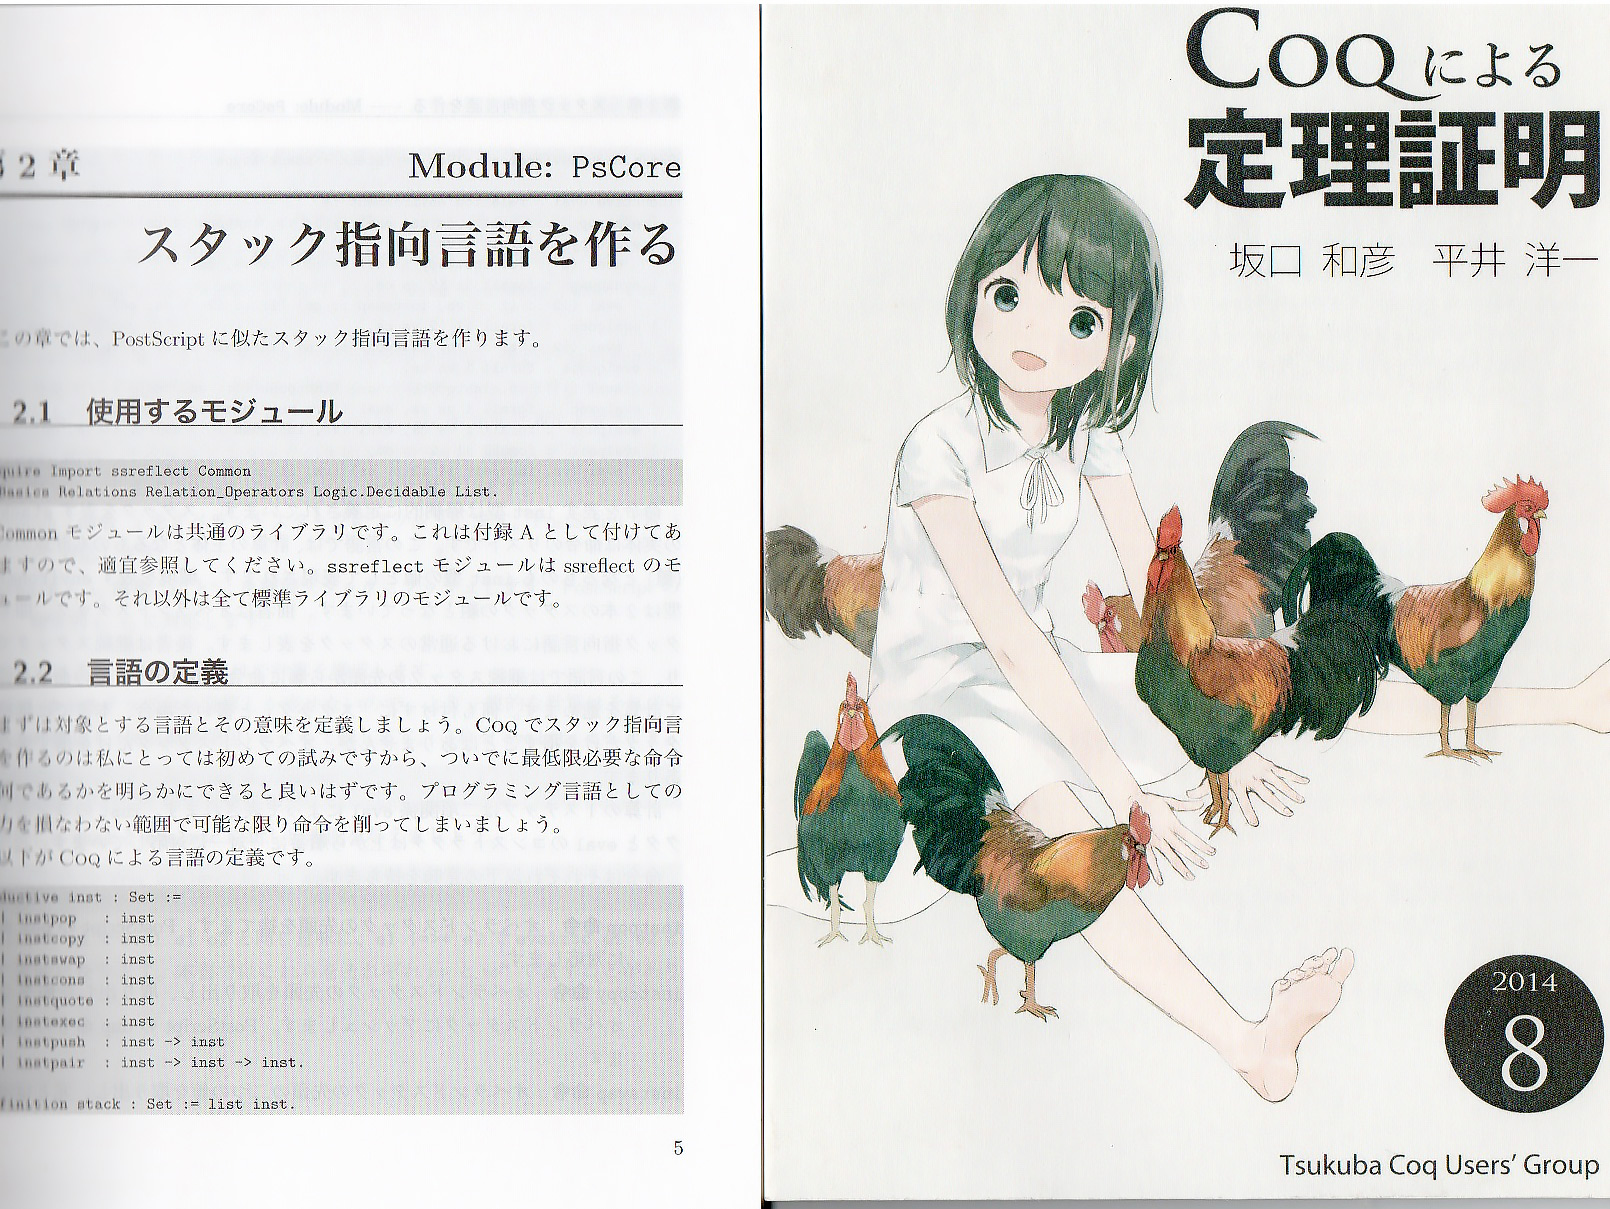
\includegraphics[height=35mm]{tsukubabooks.jpg}
%    %\includegraphics[height=45mm]{leaflet.jpg}
%      \end{block}
%      \begin{block}{\Hydras}
%        Kirby \& Paris'  hydra battles, exponentiation algorithms, \dots
%      \end{block}

% \end{frame}

%%%%%%%%%%%%%%%%%%%%%%%%%%%%%%%%%%%%%%
\begin{frame}
  \frametitle{What hydras are talking about?}
  \begin{block}{}
    \Hydras presents a consistent set of examples, which allow us to formalize 
    some \textcolor{mathcolor}{discrete math}, discuss
    \textcolor{coqstylecolor}{\coq style, specification and proof patterns}, and use\footnote{and depend on!} \textcolor{plugincolor}{a few plug-ins}.
  \end{block}
  \begin{block}{}
    \begin{description}
    \item[hydra battles:]
    
  \textcolor{mathcolor}{ordinals},
    \textcolor{mathcolor}{rapidly growing functions},
    \textcolor{mathcolor}{primitive recursive functions}, 
   \textcolor{coqstylecolor}{dependently typed functions},
    \textcolor{coqstylecolor}{operational type classes},
      \textcolor{coqstylecolor}{proofs of well-foundedness},
         \textcolor{coqstylecolor}{impossibility proofs},
    \textcolor{coqstylecolor}{uniqueness of identity proofs (UIP)},
      \textcolor{coqstylecolor}{indefinite description (Hilbert's epsilon operator)}, 
     \textcolor{plugincolor}{equations},
    \textcolor{plugincolor}{ackermann (goedel)},
      \textcolor{plugincolor}{gaia}
   
 \item[addition chains (exponentiation algorithms):]
      \textcolor{mathcolor}{algorithmics},
       \textcolor{mathcolor}{arithmetic},
            \textcolor{coqstylecolor}{operational type classes},
    \textcolor{coqstylecolor}{monadic notations},
    \textcolor{coqstylecolor}{PHOAS},
  \textcolor{coqstylecolor}{parametricity}, 
        \textcolor{plugincolor}{paramcoq}
        \end{description}
  \end{block}
\end{frame}
%%%%%%%%%%%%%%%%%%%%%%%%%%%%%%%%%%%%%%%
\section{Example: Kirby \& Paris' hydras}
\begin{frame}
  \frametitle{Example: Kirby \& Paris' hydras}
 %  \begin{block}{}
    
%   \begin{enumerate}
%   \item Intuitive presentation
%     \item From discrete math to \coq
%   \end{enumerate}
%   \end{block}

% \end{frame}
% %%%%%%%%%%%%%%%%%%%%%%%%%%%%%%%%%%%%%%%%
% \begin{frame}
%   \frametitle{The life of $\omega^{\omega^2+1}+1$}
  
  \begin{figure}[h]
  \centering
  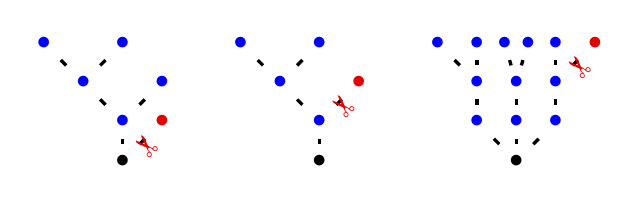
\begin{tikzpicture}[very thick, scale=0.25]
  \node (h1) at (4,0){$\bullet$};
  \node[blue] (h2) at (4,2){$\bullet$};
  \node[blue] (h3) at (2,4){$\bullet$};
  \node[blue] (h4) at (0,6){$\bullet$};
  \node[red!90!black] (h7) at (6,2){$\bullet$};
  \node[blue] (h5) at (4,6){$\bullet$};
  \node[blue] (h6) at (6,4){$\bullet$};
  \draw (h1) -- (h2) ;
  \draw (h2) -- (h3) ;
  \draw (h1) -- node[red!90!black,font=\small,sloped,shift={(0.01,-0.075)},rotate=90]{\textbf{\ding{34}}} (h7);
  \draw (h3) -- (h4) ;
  \draw (h3) -- (h5) ;
  \draw (h2) -- (h6);

  \node (h11) at (14,0){$\bullet$};
  \node[blue] (h12) at (14,2){$\bullet$};
  \node[blue] (h13) at (12,4){$\bullet$};
  \node[blue] (h14) at (10,6){$\bullet$};
  \node[blue] (h15) at (14,6){$\bullet$};
  \node[red!90!black] (h16) at (16,4){$\bullet$};
  \draw (h11) -- (h12) ;
  \draw (h12) -- (h13) ;
  \draw (h12) -- node[red!90!black,font=\small,sloped,shift={(0.01,-0.075)},rotate=90]{\textbf{\ding{34}}} (h16);
  \draw (h13) -- (h14) ;
  \draw (h13) -- (h15) ;

  
 
\node (hn1) at (24,0){$\bullet$};
\node[blue] (hn2) at (22,2) {$\bullet$};
\node[blue] (hn3) at (22,4) {$\bullet$};
\node[blue] (hn4) at (20,6){$\bullet$};
  \node[blue] (hn5) at (22,6){$\bullet$};
  \draw (hn1) -- (hn2) ;
  \draw (hn2) -- (hn3) ;
  \draw (hn3) -- (hn4) ;
  \draw (hn3) -- (hn5) ;
\node [blue](hn2b) at (24,2) {$\bullet$};
\node[blue] (hn3b) at (24,4) {$\bullet$};
\node [blue](hn4b) at (23.4,6){$\bullet$};
  \node [blue](hn5b) at (24.6,6){$\bullet$};
  \draw (hn1) -- (hn2b) ;
  \draw (hn2b) -- (hn3b) ;
  \draw (hn3b) -- (hn4b) ;
  \draw (hn3b) -- (hn5b) ;
  \node [blue](hn2c) at (26,2) {$\bullet$};
\node [blue](hn3c) at (26,4) {$\bullet$};
\node [blue](hn4c) at (26,6){$\bullet$};
  \node [red!90!black] (hn5c) at (28,6){$\bullet$};
  \draw (hn1) -- (hn2c) ;
  \draw (hn2c) -- (hn3c) ;
  \draw (hn3c) -- (hn4c) ;
  \draw (hn3c) -- node[red!90!black,font=\small,sloped,shift={(0.01,-0.075)},rotate=90]{\textbf{\ding{34}}} (hn5c) ;
\end{tikzpicture}

\caption{Three successive states of a hydra in a battle,
at time $t=0,1,2$\label{life1}}
  \label{fig:round}
\end{figure}

\begin{figure}[h]
  \centering
  
 
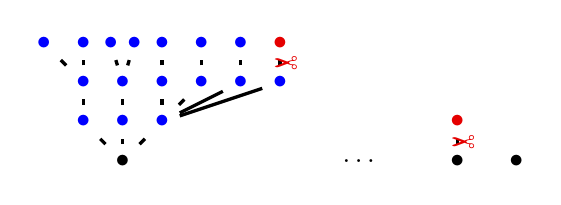
\begin{tikzpicture}[very thick, scale=0.25]
\node (hn1) at (4,0){$\bullet$};
\node[blue] (hn2) at (2,2) {$\bullet$};
\node[blue] (hn3) at (2,4) {$\bullet$};
\node[blue] (hn4) at (0,6){$\bullet$};
  \node[blue] (hn5) at (2,6){$\bullet$};
  \draw (hn1) -- (hn2) ;
  \draw (hn2) -- (hn3) ;
  \draw (hn3) -- (hn4) ;
  \draw (hn3) -- (hn5) ;
\node [blue](hn2b) at (4,2) {$\bullet$};
\node [blue](hn3b) at (4,4) {$\bullet$};
\node [blue](hn4b) at (3.4,6){$\bullet$};
  \node [blue] (hn5b) at (4.6,6){$\bullet$};
  \draw (hn1) -- (hn2b) ;
  \draw (hn2b) -- (hn3b) ;
  \draw (hn3b) -- (hn4b) ;
  \draw (hn3b) -- (hn5b) ;
  \node [blue](hn2c) at (6,2) {$\bullet$};
\node [blue](hn3c) at (6,4) {$\bullet$};
\node [blue](hn4c) at (6,6){$\bullet$};
 % \node (hn5c) at (8,6){$\bullet$};
  \draw (hn1) -- (hn2c) ;
  \draw (hn2c) -- (hn3c) ;
  \draw (hn3c) -- (hn4c) ;
  % \draw (hn3c) -- (hn5c) ;
  \node [blue](hn3d) at (8,4) {$\bullet$};
  \draw (hn2c) -- (hn3d) ;
  \node [blue](hn4d) at (8,6) {$\bullet$};
  \draw (hn3d) -- (hn4d) ;
  
 \node [blue](hn3e) at (10,4) {$\bullet$};
  \draw (hn2c) -- (hn3e) ;
  \node [blue](hn4e) at (10,6) {$\bullet$};
  \draw (hn3e) -- (hn4e) ;

  \node [blue](hn3f) at (12,4) {$\bullet$};
  \draw (hn2c) -- (hn3f) ;
  \node [red!90!black](hn4f) at (12,6) {$\bullet$};
  \draw (hn3f) -- node[red!90!black,font=\small,sloped,shift={(0.01,-0.075)},rotate=90]{\textbf{\ding{34}}} (hn4f) ;

  \node at (16,0) {$\dots$} ;

 \node [black](hn4h) at (21,0) {$\bullet$};
\node [red!90!black](hn4g) at (21,2) {$\bullet$};
   \draw (hn4h) -- node[red!90!black,font=\small,sloped,shift={(0.01,-0.075)},rotate=90]{\textbf{\ding{34}}} (hn4g) ;

  
  \node [black](hn4f) at (24,0) {$\bullet$};
\end{tikzpicture}
\caption{At $t=3,\dots,\textcolor{red}{x}-1,\textcolor{red}{x=?}$
\label{life2}}
\end{figure}
\end{frame}

\begin{frame}
  \frametitle{Mathematical formalization of hydra battles}
   \begin{block}{}
  
    \begin{itemize}
    \item   We associate a hydra to each ordinal \textcolor{mathcolor}{$\alpha<\epsilon_0$} (in Cantor normal form). For instance, the first hydra of our example is the image of \textcolor{mathcolor}{$omega^{\omega^2+1}+1$}.
    \item A round (at time $t$) of a battle transforms an hydra associated with \textcolor{mathcolor}{$\alpha$} into the hydra associated with \textcolor{mathcolor}{$\canonseq{\alpha}{t+1}$}, the $t+1$-st element of the \emph{canonical sequence} of \textcolor{mathcolor}{$\alpha$}.
    \item We want to ``compute'' the length of sequences of the form 
\textcolor{mathcolor}{$\langle \alpha_k=\alpha,\dots,\alpha_{i+1}=\canonseq{\alpha_i}{i+1},\dots, 1,0\rangle$}, where \textcolor{mathcolor}{$k\in\mathbb{N}$}.
      
  \end{itemize}
\end{block}
\end{frame}

%%%%%%%%%%%%%%%%%%%%%%%%%%%%%%%%%%%%%%%%
\begin{frame}
 
 \begin{block}{}
    Ordinals less than $\epsilon_0$ are represented as \emph{ordinal notations} which allow the user to write proofs by computation (comparison, canonical sequences, etc.)
    \begin{footnotesize}
      \inputsnippets{../../movies/snippets/ON_Generic/ONDef}

       \inputsnippets{../E0_Ex42}
    \end{footnotesize}

    
  
  \end{block}
\end{frame}

\begin{frame}
  \begin{block}{}
    \begin{itemize}
    \item We borrow the systematic study of the sequencesfrom Ketonen \& Solovay's article
      \emph{Rapidly Growing {R}amsey Functions (1981)}.

    \item Let \textcolor{mathcolor}{$0<\alpha<\epsilon_0$}, and \textcolor{mathcolor}{$i\in\mathbb{N}$}.
      The least index \textcolor{mathcolor}{$k$} such that \textcolor{mathcolor}{$\alpha_k=0$} is  \textcolor{mathcolor}{$H'_\alpha(i)$} where \textcolor{mathcolor}{$H'_\alpha$} is defined by transfinite induction over \textcolor{mathcolor}{$\alpha$}.

   %    \begin{align}
%   H'_0(i) & = i\\
%   H'_\alpha(i) &= H'_{(\canonseq{\alpha}{i+1})}(i)  \quad\textit{if $\alpha$ is a limit ordinal}\\
%   H'_{\alpha}(i) &=H'_\beta(i+1) \quad\textit{if $\alpha=\beta+1$}
% \end{align}
\vspace{5pt}
      \begin{footnotesize}
        \inputsnippets{../Hprime_HprimeDef}   
      \end{footnotesize}
      
    \end{itemize}

    
  \end{block}

  \begin{block}{}
    The \textcolor{mathcolor}{$H'_\alpha$} family is an example of \emph{hierarchy of rapidly growing functions}. For instance, \textcolor{mathcolor}{$H'_{\omega^3+3}(0)\geq2^{2^N}$}, where \textcolor{mathcolor}{$N=2^{70}-1$}.
  \end{block}
\end{frame}

 
    
 
  
   

%%%%%%%%%%%%%%%%%%%%%%%%%%%%%%%%%%%%%%%%%%%%
\begin{frame}
  \begin{block}{}
    
    Properties of the \textcolor{mathcolor}{$H'_\alpha$}s are proved with the help of the lemmas automatically generated by \textcolor{plugincolor}{equations}. For instance, the \textcolor{mathcolor}{$H'_\alpha$} are strictly monotonous, 
and if \textcolor{mathcolor}{$\beta<\alpha$}, then \textcolor{mathcolor}{$H'_\alpha(i)>H'_\beta(i)$} for all but a finite number of $i$.
  \end{block}

  
  \begin{block}{}
    We prove also that, for any   \textcolor{mathcolor}{$\alpha\geq\omega^\omega$} the function \textcolor{mathcolor}{$H'_\alpha$} is not primitive recursive.

    \begin{itemize}
    \item \emph{In order to prove this theorem, we chose to maintain under \community Russel O'Connor's library \textcolor{plugincolor}{goedel}, which contains a formalization of primitive recursive functions.}
    \item \emph{Proving formally that a given function is not primitive recursive is a nice example of application of a complex (mutually recursive, dependently typed) induction principle. You have to take into account the set of PR functions of any arity.}
      
        \item    \emph{The interest of O'Connor's contribution led us to write a chapter on primitive recursive functions, with examples and exercices.}
    \end{itemize}
  \end{block}
\end{frame}

%%%%%%%%%%%%%%%%%%%%%%%%%%%%%%%%%%%%%%%%%
\begin{frame}
  \frametitle{Some features of the \Hydras project}
  \begin{block}{}
    \begin{itemize}
    \item The order in which \coq code is presented in the book is determined by the difficulty of the mathematical examples, or the assumed level in \coq of the reader, not by the structure of the libraries.
    \item We often present and compare several different definitions and proofs of the same mathematical notions, including ``bad'' ones.
      \item We would be happy to include new proofs, if they improve old ones, or they illustrate new proof patterns. \emph{Please send PRs or issues!}.
    \end{itemize}
  \end{block}
\end{frame}
 
%%%%%%%%%%%%%%%%%%%%%%%%%%%%%%%%%%%%%%%%%


%%%%%%%%%%%%%%%%%%%%%%%%%%%%%%%%%%%%%%%%%
\begin{frame}
  \TODO{}{maintenance, CI/CD,  etc.   (several slides).}
\end{frame}
%%%%%%%%%%%%%%%%%%%%%%%%%%%%%%%%%%%%%%%
\begin{frame}
  \frametitle{Presenting proofs with \alectr}
  \begin{small}
    
 %\begin{footnotesize}
  \inputsnippets{../Schutte_Ex42a}   
 %\end{footnotesize}
 
By definition of additive principal ordinals, 
it suffices to prove the inequality $\omega+42< \phi_0(2)$.
%\begin{footnotesize}
\inputsnippets{../Schutte_Ex42b}
By Lemma \textit{AP\_plus\_closed}, it suffices to prove  $\omega<\omega^2$ and $42<\omega^2$.
%\end{footnotesize}
\end{small}

\end{frame}

\begin{frame}
  %\frametitle{Presenting proofs with \alectr (2)}
\begin{small}
%\begin{footnotesize}
\inputsnippets{
  ../Schutte_Ex42c, ../Schutte_Ex42d, ../Schutte_Ex42e}
%\end{footnotesize}
  \end{small}
  
\end{frame}
%%%%%%%%%%%%%%%%%%%%%%%%%%%%%%%%%%%%%%
\begin{frame}[fragile]
 \begin{alltt}
{\color{lightblue}{(* begin snippet Ex42a:: no-out *)}}
Example Ex42: omega + 42 + omega^2 = omega^2. 
{\color{lightblue}{(* end snippet Ex42a *)}}
Proof.
  {\color{lightblue}{(* begin snippet Ex42b *)}}
  assert (HAP:= AP_phi0 2). {\color{lightblue}{(* .no-out *)}}
  elim  HAP; intros _ H0; apply H0; clear H0. 
  {\color{lightblue}{(* end snippet Ex42b *)}}
  {\color{lightblue}{(* begin snippet Ex42d *)}}
  Check AP_plus_closed. {\color{lightblue}{(* .unfold .no-goals *)}}
  {\color{lightblue}{(* end snippet Ex42d *)}}
   {\color{lightblue}{(* begin snippet Ex42c *)}}
  assert (Hlt: omega < omega^2) by 
      (rewrite omega_eqn; apply phi0_mono, finite_mono;
        auto with arith).
 {\color{lightblue}{ (* end  snippet Ex42c *)}}
\end{alltt}
\end{frame}
%%%%%%%%%%%%%%%%%%%%%%%%%%%%%%%%%%%%%%%%%%
\begin{frame}
  \frametitle{Perspectives}
  \begin{block}{Library on ordinals}
    \begin{itemize}
    \item \TODO{}{Gaia}
      \item \TODO{}{Aczel, Minki}
    \end{itemize}
  \end{block}
\end{frame}

%%%%%%%%%%%%%%%%%%%%%%%%%%%%%%%%%%%%%%%%%%%%
\begin{frame}
  \frametitle{Perspectives(2)}
  \begin{block}{Documentation with Alectryon}
    \begin{itemize}
    \item \TODO{}{}
    \end{itemize}
  \end{block}
\end{frame}
%%%%%%%%%%%%%%%%%%%%%%%%%%%%%%%%%%%%%%%%%%%%
\begin{frame}
  \frametitle{Perspectives(3)}
  \begin{block}{CI/CD}
     \TODO{}{}
  \end{block}
\end{frame}
%%%%%%%%%%%%%%%%%%%%%%%%%%%%%%%%%%%%%%%%%%%

\begin{frame}
  \frametitle{Conclusion}
  \begin{block}{}
    \begin{itemize}
    \item \TODO{}{}
    \item \Hydras and \community are on github. Please contribute!
      \begin{itemize}
    \item New chapters
    \item Any improvement (text and/or proofs)
    \end{itemize} 
    \end{itemize}
 \end{block}

\end{frame}

\end{document}

